\chapter{Lossy Passive Relays}
\label{sec:lossyrel}

In this chapter, the effect of lossy passive relays will be explored.
In the beginning we justified the choice of considering only pure imaginary impedances at the relays, by the fact, that this results in loss less relays.
In the following we will allow the impedances to become complex, with a strict positive real part, i.e.
$\mat{Z}_\text{Rel} = \mat{R}_\text{Rel} + j\mat{X}_\text{Rel}$ with $R_\text{Rel}[i]>=0,\forall i\in[1,\cdots,N_{Rel}]$.

It is obvious, that the performance of this system must be strictly larger than allowing only loss less relays, as we can set the real part to zero and therefore we would get the same result.

\begin{figure}[h]
\centering
  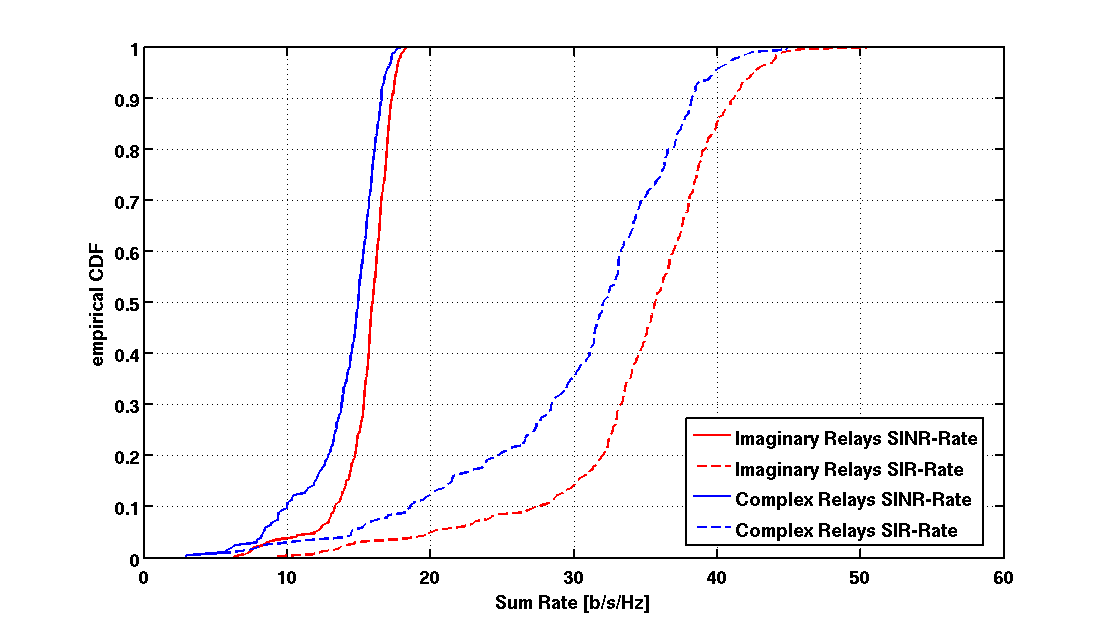
\includegraphics[width=\linewidth]{images/Imagvscomp.png}
\caption{Comparison of loss less and lossy relays.}
\label{fig:lossyrel}
\end{figure}

Figure~\ref{fig:lossyrel} shows the performance of the loss less relays in red, as we know them from the previous chapters.
In blue the performance of the lossy relays is given.
We see, that the performance is lower than the performance of the loss less relays, which is contradicting to the statement above.
This leads to the conclusion, that the performance of the solver is worse, when the degree of freedom is larger.
Approaches to prevent the solver in running into these lower rates would be a pre-optimization of the loss less relays and afterwards performing an optimization with lossy relays using the results from the red curve as initial values.



\chapter{Nossek}
\label{sec:nossek}

As written in the Introduction of this thesis, the circuit description is based on the methods introduced in~\cite{Nossek}.

\section{Transfer Function}
To be able to fully use this method some adoptions need to be made.
In~\cite{Nossek}, the use of relays was not introduced.
In order to use the description, we model the relays as receivers with the following setting for the matching network:	
\begin{align}
\label{eq:nossek_matching}
\mat{Z}_\text{M11}[N_\text{R}\cdot N_\text{Rx}+\left(1:N_\text{Relay}\right)] &=
	\text{diag}\left(\vec{Z}_\text{Relay}\right)\\
\mat{Z}_\text{M12}[N_\text{R}\cdot N_\text{Rx}+\left(1:N_\text{Relay}\right)] &= 
	\mat{Z}_\text{M21}[N_\text{R}\cdot N_\text{Rx}+\left(1:N_\text{Relay}\right)] = \mat{0}\\
\mat{Z}_\text{M22}[N_\text{R}\cdot N_\text{Rx}+\left(1:N_\text{Relay}\right)] &= \text{undef.}%\\
%\mat{Z}_\text{M11} &=
%\begin{bmatrix}
%\text{M}_\text{1,11} & \cdots & 0 &\\
% \vdots & \ddots & \vdots & \mat{0} \\
% 0 & \cdots & \text{M}_\text{M,11}&\\
% & \mat{0}& & \text{diag}\left(\mat{s}\right)
%\end{bmatrix}\\
%\mat{Z}_\text{M12}&=
%\begin{bmatrix}
%\text{M}_\text{1,12} & \cdots& 0&\\
%\vdots & \ddots & \vdots & \mat{0}\\
%0 & \cdots & \text{M}_\text{M,12}&\\
%& \mat{0} &	& 0\cdot\mat{I}_{N_\text{Relays}}
%\end{bmatrix}
\end{align}

The equivalent input impedance matrix for the relay ports hence becomes
\begin{align}
\label{eq:nossek_matching}
\mat{Z}_\text{inM}[N_\text{R}\cdot N_\text{Rx}+\left(1:N_\text{Relay}\right)] &= \text{diag}\left(\vec{Z}_\text{Relay}\right).
\end{align}
\subsection{Signal Transfer Function}
The circuitry transfer function from~\cite{Nossek} applied to the adoptions, leads to
\begin{align}
\label{eq:nossek_transf}
\mat{H}_\text{L,A} &= \frac{z_l d}{z_l + g}\mat{D}\mat{F}_\text{R},\quad\text{with}\\
\label{eq:nossek_D}
\mat{D} &= \left(c\mat{I} + \mat{Z}_\text{R}\right)^{-1},\\
\label{eq:nossek_F}
\mat{F}_\text{R} &= \mat{Z}_\text{M12}\left(\mat{Z}_\text{M11}+\mat{Z}_\text{C}\right)^{-1},\quad\text{and}\\
\label{eq:nossek_Zr}
\mat{Z}_\text{R} &= \mat{Z}_\text{M22} + \mat{F}_\text{R}\mat{Z}_\text{M12}.
\end{align}
Note, that in~\cite{Nossek}, the matching network is defined differently, i.e. $\mat{Z}_\text{M11}$ and $\mat{Z}_\text{M22}$ are swapped.
$\mat{H}_\text{L,A}$ denotes hereby the transfer function from all the open circuit input voltages to all the voltages over the downstream circuitry loads.
To get the transfer function only towards receiver $j$, only the rows $\left[(j-1)\cdot N_\text{Rx}+1 : j\cdot N_\text{Rx}\right]$ must be considered.
In the following we denote such case by $\mat{H}_{\text{L,}j}$ and we can write the overall transfer function by
\begin{align}
%\vec{v}_\text{L} &= \mat{H}_\text{L,0}\cdot\vec{v}_o + \vec{n}\\
\vec{v}_{\text{L},j}^s &= \mat{H}_{\text{L,}j}\cdot\mat{H}_{j}^{\text{sp}}\cdot\vec{v}_j.
\end{align}

\subsection{Noise Transfer Function}
Similarly, the new model can be applied to the noise sources.
According to~\cite[Equation (14)]{Yahia2013}, this leads to the transfer function
\begin{align}
\vec{v}_{\text{L},j}^n &= \frac{z_l d}{z_l +g}\left(\mat{D}\left(\mat{Z}_\text{R}\vec{i}_\text{LNA} - \vec{v}_\text{LNA} +\mat{F}_\text{R}\vec{n}_\text{AR}\right) + \frac{1}{d}\vec{\tilde{v}}_n\right).
\end{align}
Compared to the sources introduced in Section~\ref{sec:noise_description}, the noise contribution for the LNA and the downstream used in this formula must be extended by the length of $N_\text{Relay}$ with zeros, to form a valid matrix multiplication.
As in the previous section the index $j$ denotes the branches of the j-th receiver, i.e. the rows $\left[(j-1)\cdot N_\text{Rx}+1 : j\cdot N_\text{Rx}\right]$ of the transfer function matrix.

\section{Analytical Gradient}
In the following the analytical gradient will be derived.
In contrast to Chapter~\ref{sec:ana_grad}, the rate is only dependent on $\mat{Z}_{\text{M}ij},$ with $i,j\in\{1,2\}$, as the relays were expressed by the matching network as written above.
Therefore, similar to~\cite{Yahia2013}, with the adoptions to the matching network it follows
\begin{align}
\label{eq:gradient}\nonumber
\frac{\partial r}{\partial\mat{Z}_{\text{M},ij}} &= \frac{1}{\text{ln}(2)} 
\text{Tr}\Bigg(\left(\mat{K}_s + \mat{K}_i + \mat{K}_n\right)^{-1}
\left(\frac{\partial\mat{K}_s}{\partial\mat{Z}_{\text{M},ij}}+
 \frac{\partial\mat{K}_i}{\partial\mat{Z}_{\text{M},ij}}+
 \frac{\partial\mat{K}_n}{\partial\mat{Z}_{\text{M},ij}}\right)-\\
 &\quad\left(\mat{K}_i+\mat{K}_n\right)^{-1}
 \left(\frac{\partial\mat{K}_i}{\partial\mat{Z}_{\text{M},ij}}+
 	\frac{\partial\mat{K}_n}{\partial\mat{Z}_{\text{M},ij}}\right)\Bigg).
\end{align}
The derivations of the rate with no interference can be found in~\cite{Yahia2013}.
To get the gradient of the interference, the sum over all interferer is taken, as in Section~\ref{sec:int_cov}.


%MU-MIMO TF

%\begin{align}
%\label{eq:nossek_transf}
%\vec{y}_i &= \mat{A}_{i,i}\vec{x}_i + 
%	\sum_{j=0,j\neq i}^{N_\text{User}-1} \mat{A}_{i,j}\vec{x}_j + \vec{n}\\
%\mat{A} &= \mat{H}_\text{L,0}\cdot\mat{H}^{\text{sp}}
%\end{align}

%User 0 achievable rate:
%\begin{align}
%\label{eq:achiev_rate}
%r_i &= \text{log}_2\left(\text{det}\left(\mat{K}_{\text{s},i}\left(\mat{K}_{\text{i},i}+\mat{K}_{\text{n},i}\right)^{-1}+\mat{I}_{N_\text{R}}\right)\right)\\
% &=\text{log}_2\left(
%	\text{det}\left(\mat{K}_{\text{s},i}+
%		\mat{K}_{\text{i},i}+\mat{K}_{\text{n},i}\right)\right) -
%	\text{log}_2\left(\text{det}\left(\mat{K}_{\text{i},i}+\mat{K}_{\text{n},i}\right)\right).
%\end{align}

%Signal Cov
%\begin{align}
%\mat{K}_{\text{s},i}=\mathbb{E}[\vec{v}_\text{L}^\text{s}\vec{v}_\text{L}^{\text{s}^H}] &= 
%	\mat{H}_\text{L,0} \cdot \mat{H}_{i}^{\text{sp}} \cdot 
%	\mathbb{E}[\vec{v}_{i}\vec{v}_{i}^H] \cdot 
%	\mat{H}_{i}^{\text{sp}^H} \cdot \mat{H}_\text{L,0}^H,\\
%\mat{K}_{\text{s},i}=\mathbb{E}[\vec{v}_\text{L}^\text{s}\vec{v}_\text{L}^{\text{s}^H}] &= 
%	\mat{H}_\text{L,0} \cdot \mat{H}_{i}^{\text{sp}} \cdot  
%	\mat{H}_{i}^{\text{sp}^H} \cdot \mat{H}_\text{L,0}^H\cdot P_i
%\end{align}
%Interference Cov
%\begin{align}
%\mat{K}_{\text{i},i}=\mathbb{E}[\vec{v}_\text{L}^\text{i}\vec{v}_\text{L}^{\text{i}^H}] &= \sum_{j=0,j\neq i}^{N_\text{User}-1} 
%	\mat{H}_\text{L,0} \cdot \mat{H}_{j}^{\text{sp}} \cdot 
%	\mathbb{E}[\vec{v}_{j}\vec{v}_{j}^H] \cdot 
%	\mat{H}_{j}^{\text{sp}^H} \cdot \mat{H}_\text{L,0}^H,\\
%	&= \mat{H}_\text{L,0} \left(\sum_{j=1}^{N_\text{User}-1} 
%	\cdot \mat{H}_{j}^{\text{sp}} \cdot 
%	\mathbb{E}[\vec{v}_{j}\vec{v}_{j}^H] \cdot 
%	\mat{H}_{j}^{\text{sp}^H}\right) \cdot \mat{H}_\text{L,0}^H,\\
%\mat{K}_{\text{i},i}=\mathbb{E}[\vec{v}_\text{L}^\text{i}\vec{v}_\text{L}^{\text{i}^H}] &= \sum_{j=0,j\neq i}^{N_\text{User}-1} 
%	\mat{H}_\text{L,0} \cdot \mat{H}_{j}^{\text{sp}} \cdot 
%	\mat{H}_{j}^{\text{sp}^H} \cdot \mat{H}_\text{L,0}^H\cdot P_j,\\
%	&= \mat{H}_\text{L,0} \left(\sum_{j=1}^{N_\text{User}-1} 
%	\cdot \mat{H}_{j}^{\text{sp}} \cdot
%	\mat{H}_{j}^{\text{sp}^H}\right) \cdot \mat{H}_\text{L,0}^H\cdot P_j
%\end{align}

